%%%%%%%%%%%%%%%%%%%%%%%%%%%%%%%%%%%%%%%%%%%%%%%%%%%%%%%%%%%%%%%%%%%%%%
%%%%%%%%%%%%%%%%%%%%%%%%%%%%%%%%%%%%%%%%%%%%%%%%%%%%%%%%%%%%%%%%%%%%%%
%%%%%%%%%%%%%%%%%%%%%%%%%%%%%%%%%%%%%%%%%%%%%%%%%%%%%%%%%%%%%%%%%%%%%%
\newpage
\section{Other Panel Integrals}
\begin{figure}
\resizebox{\textwidth}{!}{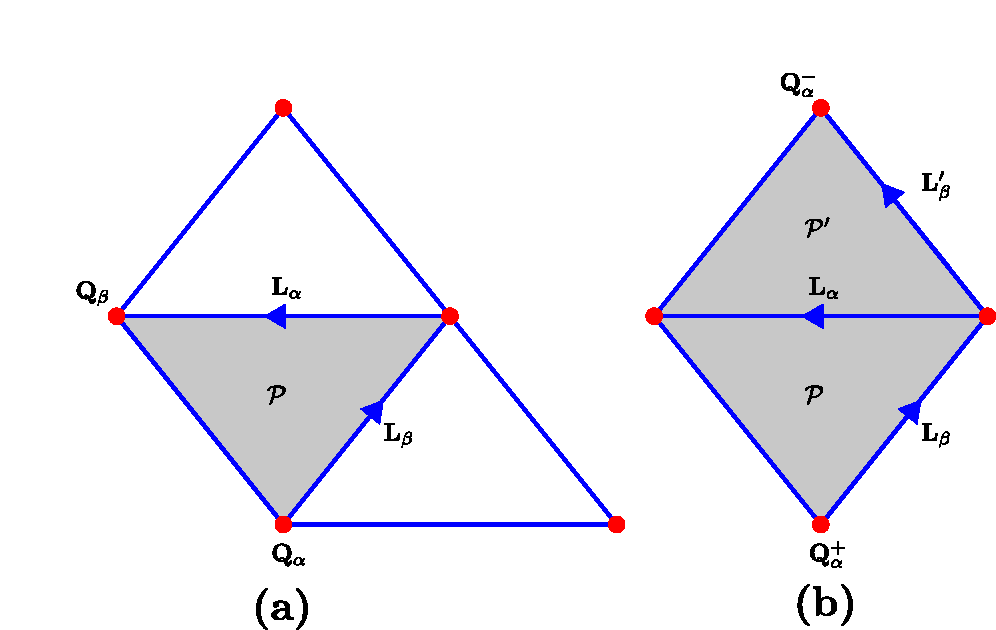
\includegraphics{OverlapIntegrals.pdf}}
\caption{Notation for computation of overlap integrals.}
\label{OverlapIntegralFigure}
\end{figure}

\subsection{Overlap Integral}

The overlap integral between two RWG basis functions is 
$$ O_{\alpha\beta}=
\Big<\vb f_\alpha \Big | \vb f_\beta\Big > 
=\int_{\text{\scriptsize sup }\vb f_\alpha\, \cap \,
        \text{\scriptsize sup }\vb f_\beta } 
  \vb f_\alpha(\vb x) \cdot \ \vb f_\beta(\vb x)
   \,d\vb x.
$$
If we think of $O_{\alpha\beta}$ as the $\alpha,\beta$ element of 
a matrix $\vb O$, then $\vb O$ is a very sparse matrix, with
at most 5 nonzero entries per row. Fix an interior edge 
$\vb L_\alpha$ in a triangular surface mesh and consider the 
basis function $\vb f_\alpha$ associated with this edge.
The only basis functions to have nonvanishing overlap with 
$\vb f_\alpha$ are \textbf{(1)} $\vb f_\alpha$ itself, and 
\textbf{(2)} basis functions associated with the four 
edges beside $\vb L_\alpha$ on the two panels that 
share $\vb L_\alpha$, such as $\vb L_\beta$ in Figure 
\ref{OverlapIntegralFigure}\textbf{(a)}.

\paragraph{The case $\alpha\ne \beta$.} 

Consider first the case of inequal basis functions
$\vb f_\alpha,\vb f_\beta$ that share a single
panel $\mathcal{P}$ [Figure \ref{OverlapIntegralFigure}\textbf{(a)}].
We parameterize points within $\mathcal{P}$ 
according to 
$$ \vb x=\vb Q_\alpha + u\vb L_\beta + v\vb L_\alpha, 
   \qquad 0\le u \le 1, \quad 0 \le v \le u.
$$
On $\mathcal{P}$, the two basis functions may be expressed in 
terms of this parameterization as 
\begin{align*} 
 \vb f_\alpha(\vb x) 
&= 
 \frac{\sigma^\alpha l_\alpha}{2A}
 \Big[u\vb L_\beta + v\vb L_\alpha\Big] 
\\
 \vb f_\beta(\vb x) 
&= \frac{\sigma^\beta l_\beta}{2A}
  \Big[ u\vb L_\beta + v\vb L_\alpha + (\vb Q_\alpha - \vb Q_\beta)\Big]
\\
&= \frac{\sigma^\beta l_\beta}{2A}
  \Big[ (u-1)\vb L_\beta + (v-1)\vb L_\alpha\Big]
\end{align*} 
Here $A$ is the area of $\mathcal{P}$ and $\sigma^\alpha = \pm 1$  
according as $\mathcal{P}$ is the positive or negative panel
associated with basis function $\vb f_\alpha$ (and similarly 
for $\sigma^{\beta}$), and we used the fact that 
$\vb Q_\alpha + \vb L_\beta + \vb L_\alpha = \vb Q_\beta.$

The overlap integral is 
\begin{align}
O_{\alpha\beta}
&=\int_{\mathcal{P}} \vb f_\alpha(\vb x) \cdot \vb f_\beta(\vb x)  \, d\vb x 
\nn
&=\frac{\sigma^\alpha \sigma^\beta l_\alpha l_\beta}{2A} 
  \int_0^1 \, du \, \int_0^u \, dv \, 
  \Big[ u \vb L_\beta + v\vb L_\alpha\Big]
 \cdot
  \Big[ (u-1) \vb L_\beta + (v-1)\vb L_\alpha\Big]
\nn
&=-\frac{\sigma^\alpha \sigma^\beta l_\alpha l_\beta}{24A} 
  \Big[ l_\alpha^2 + l_\beta^2 + 3\vb L_\alpha\cdot \vb L_\beta\Big]
\label{OAlphaBeta}
\end{align}

\paragraph{The case $\alpha=\beta$.}

In this case there are two panels that contribute
[Figure \ref{OverlapIntegralFigure}\textbf{(b)}].
The contribution of $\mathcal{P}$ is
\begin{align*}
\int_{\mathcal{P}} \vb f_\alpha(\vb x) \cdot \vb f_\alpha(\vb x)  \, d\vb x 
&=\frac{l_\alpha^2}{2A} 
  \int_0^1 \, du \, \int_0^u \, dv \, 
  \Big[ u \vb L_\beta + v\vb L_\alpha\Big]
 \cdot
  \Big[ u \vb L_\beta + v\vb L_\alpha\Big]
\\
&=\frac{l^2_\alpha}{24A} 
  \Big[ 3l_\alpha^2 + l_\beta^2 + 3\vb L_\alpha\cdot \vb L_\beta\Big].
\end{align*}
Adding the contribution of $\mathcal{P}^\prime$, 
the total overlap integral is 
\numeq{OAlphaAlpha}
{
O_{\alpha\alpha}
=\frac{l^2_\alpha}{24}
 \bigg\{ 
   \frac{1}{A}        \Big[ l_\alpha^2 + 3l_\beta^2 + 3\vb L_\alpha\cdot \vb L_\beta\Big]
 + \frac{1}{A^\prime} \Big[ l_\alpha^2 + 3l_\beta^{\prime 2} 
                            + 3\vb L_\alpha\cdot \vb L_\beta^\prime\Big]
 \bigg\}.
}

\subsection{Crossed Overlap Integral}

The crossed overlap integral between two RWG basis functions is 
$$ O^{\times}_{\alpha\beta}=
\Big<\vb f_\alpha \Big | \vbhat{n}\times \vb f_\beta\Big > 
=\int_{\text{\scriptsize sup }\vb f_\alpha\, \cap \,
        \text{\scriptsize sup }\vb f_\beta } 
  \vb f_\alpha(\vb x) \cdot \Big[\vbhat{n}(\vb x)\times  \vb f_\beta(\vb x)\Big]
   \,d\vb x
$$
where $\vbhat{n}(\vb x)$ is the surface normal at $\vb x$. 
(The direction of $\vbhat{n}$ must be chosen consistently; 
in {\sc libscuff} this is done by placing one or more 
\textit{reference points} inside closed objects and choosing 
the surface normal to each panel to point \textit{away}
from the nearest reference point.)

$ O^{\times}_{\alpha\beta}$ is only nonzero in 
the case of Figure \ref{OverlapIntegralFigure}\textbf{(b)}.
(In particular, the diagonal element 
$ O^{\times}_{\alpha\alpha}$ vanishes.)
Proceeding in analogy to the computation leading to 
equation (\ref{OAlphaBeta}), we find
\begin{align}
O^{\times}_{\alpha\beta}
&=\int_{\mathcal{P}} \vb f_\alpha(\vb x) \cdot 
                     \Big[\vbhat{n} \times \vb f_\beta(\vb x)\Big]  \, d\vb x 
\nn
&=\frac{\sigma^\alpha \sigma^\beta l_\alpha l_\beta}{2A} 
  \int_0^1 \, du \, \int_0^u \, dv \, 
  \Big[ u \vb L_\beta + v\vb L_\alpha\Big]
 \cdot
  \Big[ (u-1) \big(\vbhat{n}\times \vb L_\beta\big) + 
        (v-1) \big(\vbhat{n}\times \vb L_\alpha\big)
  \Big]
\nn
&=\frac{\sigma^\alpha \sigma^\beta l_\alpha l_\beta}{12A} 
  \Big[ \vb L_\alpha \cdot (\vbhat{n}\times \vb L_\beta) \Big]
\nn
&=\frac{\sigma^\alpha \sigma^\beta l_\alpha l_\beta}{12A} 
  \Big[ \vbhat{n} \cdot \big(\vb L_\beta\times \vb L_\alpha\big) \Big]
\nonumber
\intertext{by cyclic permutation of the triple vector product. But
the magnitude of the cross product here is just $\vbhat{n}$ times 
twice the panel area,}
&=\frac{\sigma^\alpha \sigma^\beta l_\alpha l_\beta}{12A} 
  \Big[ \vbhat{n} \cdot \big(\pm 2A\,\vbhat{n}\big) \Big]
\nn
&=\pm\frac{\sigma^\alpha \sigma^\beta l_\alpha l_\beta}{6}.
\label{OTimesAlphaBeta}
\end{align}
The $\pm$ sign is determined as follows: Suppose we start 
at vertex $\vb Q_\alpha$ and traverse the vertices of 
$\mathcal{P}$ by following $\vb L_\beta$, then $\vb L_\alpha$.
If in so doing we encounter the vertices of $\pan$ in 
the order $(0,1,2)$ or a cyclic permutation thereof, then
the $+$ sign holds in (\ref{OTimesAlphaBeta}); otherwise
(i.e. if we encounter the vertices in the order $(0,2,1)$ or 
a cyclic permutation thereof) the $-$ sign holds.

An easy way to determine this sign is to look at the 
indices within $\mathcal{P}$ of vertices $\vb Q_\beta$
and $\vb Q_\alpha$. Call these $I_\pan(\vb Q_\beta)$ and 
$I_\pan(\vb Q_\alpha)$, respectively; they are integers
defined modulo 3. Then the sign in (\ref{OTimesAlphaBeta})
is 
$$ \text{sign in equation (\ref{OTimesAlphaBeta})} 
   = 
   \begin{cases}
   +, \quad &\text{if } I_\pan(\vb Q_\beta)
                       -I_\pan(\vb Q_\alpha)
                        \equiv 2 \text{ mod } 3 
   \\
   -, \quad &\text{if } I_\pan(\vb Q_\beta)
                       -I_\pan(\vb Q_\alpha)
                        \equiv 1 \text{ mod } 3.
   \end{cases}
$$

%%%%%%%%%%%%%%%%%%%%%%%%%%%%%%%%%%%%%%%%%%%%%%%%%%%%%%%%%%%%%%%%%%%%%%
%%%%%%%%%%%%%%%%%%%%%%%%%%%%%%%%%%%%%%%%%%%%%%%%%%%%%%%%%%%%%%%%%%%%%%
%%%%%%%%%%%%%%%%%%%%%%%%%%%%%%%%%%%%%%%%%%%%%%%%%%%%%%%%%%%%%%%%%%%%%%
\newpage
